\documentclass[12pt]{article}

\usepackage{amsmath}

\usepackage{graphicx}
\usepackage{pgfplots}
\usepackage{hyperref}
\usepackage{amsmath}
\usepackage{amssymb}
\usepackage[bb=boondox]{mathalfa}

\usepackage[utf8]{inputenc}
\usepgfplotslibrary{colorbrewer}
\pgfplotsset{width=7cm,compat=1.18}

\title{Algèbre Linéaire}

\date{Automne 2023}

\begin{document}

\maketitle

\newcommand{\R}{\mathbb{R}}
\newcommand{\K}{\mathrm{K}}
\newcommand{\C}{\mathbb{C}}
\newcommand{\zero}{\mathbb{0}}
\newcommand{\family}{\{v_i\}_{i\in I}}
\newcommand{\uv}{\{u,v\}}

Ce document est une tentative de polycopié pour le cours d'algèbre 
linéaire I d'automne 2023 11M010. Tous les exemples du cours n'y figurent pas, mais tout le reste y est (ou devrait y être).
\\
Si vous trouvez une erreur (il y en a (plein)), faites une pull request sur github ou contactez-moi sur Telegram (alternis).
\\
Liste des cours inclus dans le document :
\begin{itemize}
    \item Cours du 21.9
    \item Cours du 22.9
    \item Cours du 28.9
\end{itemize}
\pagebreak
\tableofcontents
\pagebreak

\section*{Motivation}
On souhaite résoudre un système d'équations linéaires.
\subsection*{Exemple 1}
Une équation linéaire à 1 inconnue de la forme :
$$
ax+b=c
$$
Ici, $x$ est l'inconnue et $a,b,c \in \R$ des constantes. On souhaite trouver $Sol \subset \R$
l'ensemble des solutions.
$$
Sol = \begin{cases} \{\frac{c-b}{a}\}, \text{ si a} \neq 0 \\
     \R, \text{ si a}=0 \text{ et } b = c \\ 
    \emptyset, \text{ si a}=0 \text{ et } b \neq c
    \end{cases}
$$
\subsection*{Définition 1}
Un système à $m$ équations linéaires à $n$ variables à 
coefficients réels* est constitué de $m$ équations de la forme :

$$
\begin{aligned}
    a_{11}x_1 + a_{12}x_2 + \dots + a_{1n}x_n &=b_1 \\
    & \vdots \\
    a_{m1}x_1 + a_{m2}x_2 + \dots + a_{mn}x_n &=b_m \\
\end{aligned}
$$
Les coefficients du système sont $a_{11}, \dots, a_{1n}, \dots, a_{m1}, \dots, a_{mn}$.
On appelle les coefficients $b_1, \dots, b_m$ les "coefficients libres".
Dans le cas particulier où $b_1 = \dots = b_m$, on dit que le système est \textbf{homogène}.

\textit{*On parle aussi de systèmes à coefficients complexes. Ils sont abordés plus loin, dans le chapitre X.}

Résoudre un tel système revient à trouver son ensemble de solutions $Sol$.
$$Sol = \{(\alpha_1, \dots, \alpha_n) \text{ où } \alpha_i \in \R, i = 1, \dots, n\}$$
\pagebreak
\section{Chapitre 1 - Espaces vectoriels}
\subsection{Définitions, exemples et propriétés}
Pour motiver la définition, on considère quelques exemples de systèmes linéaires.
\subsubsection*{Exemple a)}
$n=2, m=2$
$$\begin{aligned}
\begin{cases}
    x+2y = 2 \\
    x-y=-4
\end{cases}
\\
x = -4+y \Rightarrow 3y = 6 \Rightarrow \begin{cases} y = 2 \\ x = -2 \end{cases}
\\
Sol = \{(-2, 2)\}
\end{aligned}
$$
Cette solution a un sens géométrique : les droites d'équations décrites dans le systèmes se croisent bien au point $(-2, 2)$.
\\
\begin{center}
    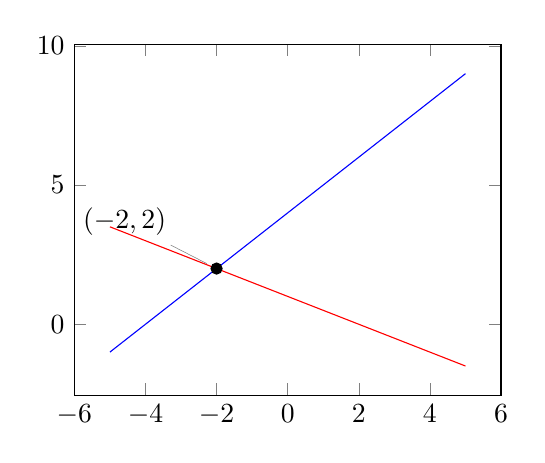
\begin{tikzpicture}
        \begin{axis}
        \addplot[color=red]{-0.5*x+1};
        \addplot[color=blue]{x+4};
        \addplot[mark=*] coordinates {(-2,2)} node[pin=150:{$(-2,2)$}]{} ;
        \end{axis}
        \end{tikzpicture}
\end{center}
\pagebreak
\subsubsection*{Exemple b)}
$n=2, m=2$
$$
\begin{cases}
    x+2y = 2 \\
    x+2y= 0
\end{cases} \Rightarrow Sol = \emptyset
$$
Les droites ne se croisent effectivement jamais.
\begin{center}
    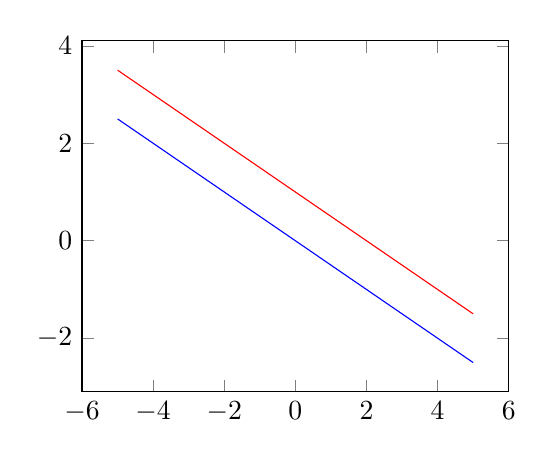
\begin{tikzpicture}
        \begin{axis}
        \addplot[color=red]{1-0.5*x};
        \addplot[color=blue]{-0.5*x};
        \end{axis}
        \end{tikzpicture}
\end{center}
\pagebreak
\subsubsection*{Exemple c)}
$n=2, m=2$
$$
\begin{cases}
    x+2y = 0 \\
    2x+y= 0
\end{cases} \Rightarrow Sol = \{(0,0)\}
$$
Ce système est homogène. 
\begin{center}
    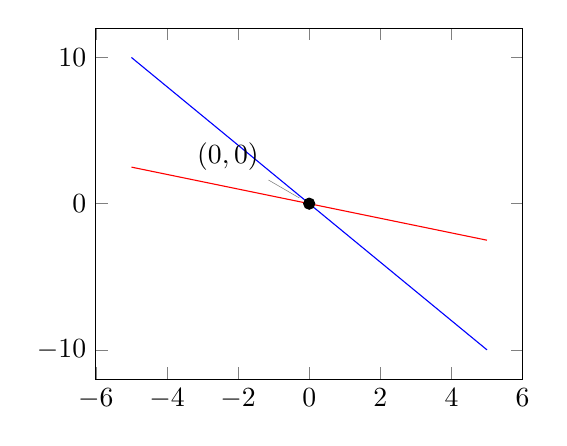
\begin{tikzpicture}
        \begin{axis}
        \addplot[color=red]{-0.5*x};
        \addplot[color=blue]{-2*x};
        \addplot[mark=*] coordinates {(0,0)} node[pin=150:{$(0,0)$}]{} ;
        \end{axis}
        \end{tikzpicture}
\end{center}
\pagebreak
\subsubsection*{Exemple d)}
$$
\begin{cases}
    x+2y=0
    \\
    2x+2y=0
\end{cases} \Rightarrow Sol = \{(x,y) \in \R^2 : y = - \frac{x}{2}\}
$$
\begin{center}
    \begin{tikzpicture}
        \begin{axis}
        \addplot[color=red]{-0.5*x};
        \addplot[color=blue]{-0.5*x};
        \end{axis}
        \end{tikzpicture}
\end{center}
Les deux droites sont superposées, l'ensemble des solutions prend donc la forme d'une droite.
\pagebreak
\subsubsection*{Exemple e)}
Ici, $m=3, n=2$.
$$
\begin{cases}
    x+2y = 0
    \\
    2x+y = 0
    \\
    x-y = 5
\end{cases} = \emptyset    
$$

\begin{center}
    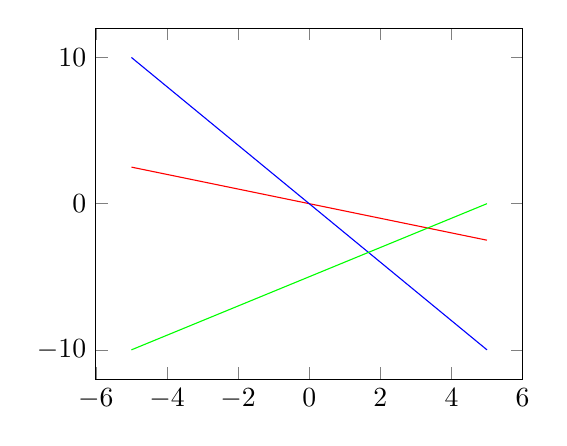
\begin{tikzpicture}
        \begin{axis}
        \addplot[color=red]{-0.5*x};
        \addplot[color=blue]{-2*x};
        \addplot[color=green]{x-5};
        \end{axis}
        \end{tikzpicture}
\end{center}
Il n'y a pas de solution, puisqu'il n'existe aucun point d'intersection des trois droites.

\pagebreak
\subsection{Propriétés des solutions de systèmes homogènes}
On observe que l'ensemble de solutions d'un système homogène à $m$ équations et $n$ inconnues satisfait les trois propriétés suivantes :
\begin{enumerate}
    \item $\alpha_1 = 0, \dots, \alpha_n = 0$ est toujours une solution.
    \item si $(\alpha_1, \dots, \alpha_n)$ et $(\alpha_1', \dots, \alpha_n')$ 
    sont deux solutions, alors leur somme $(\alpha_1+\alpha_1', \dots, \alpha_n+\alpha_n')$ est aussi une solution.
\end{enumerate}
\subsubsection{Démonstration de la propriété 2}
Soit $i \in \{1, \dots, m\}$.
$$\begin{aligned}
a_{i1}(\alpha_1+\alpha_1') + \dots + a_{in}(\alpha_n+\alpha_n')
\end{aligned}
$$
On a remplacé les facteurs $(x_1, \dots, x_n)$ par les solutions supposées.
Par distributivité, on obtient :
$$\begin{aligned}
    &a_{i1}\alpha_1 + a_{i1}\alpha_1' + \dots + a_{in}\alpha_n + a_{in}\alpha_n' \\
    &= (a_{i1}\alpha_{1}+a_{i2}\alpha_2+\dots+a_{in}\alpha_n) + (a_{i1}\alpha_{1}'+\dots+a_{in}\alpha_n') \\
    &= 0 
\end{aligned}
$$
Or, on sait déjà que $(\alpha_1, \dots, \alpha_n)$ et $(\alpha_1', \dots, \alpha_n')$ sont des solutions. On peut en conclure que leur addition donne également zéro, et que notre solution supposée $(\alpha_1 + \alpha_1', \dots, \alpha_n + \alpha_n')$ en est bien une.

On peut prouver la propriété 3) de la même façon.

\pagebreak
\subsection{Définition - Espace vectoriel}
Un \textbf{espace vectoriel réel} est un ensemble $V$ muni de deux opérations :
\begin{enumerate}
    \item "addition" : $V \times V \rightarrow V, (v, v') \rightarrow v + v'$
    \item "multiplication par un scalaire" : $\R \times V \rightarrow V, (\alpha, v) \rightarrow \alpha \cdot v$ 
\end{enumerate}

Ces deux opérations doivent satisfaire une liste d'axiomes pour que l'ensemble soit un espace vectoriel.
\begin{itemize}
    \item $\forall u,w,u \in V$, on a $(u+w)+u=v+(w+u)$, l'associativité de l'addition.
    \item $\forall u,w \in V, v+w = w+v$, commutativité de l'addition
    \item Il existe un élément noté $\zero \in V$ tel que $\zero +v = v \quad \forall v \in V$
    \item $\forall v \in V \space \exists -v : v + (-v) = \mathbb 0$
    \item $\alpha * (u+v) = \alpha*u+\alpha*v \space \forall \alpha \in \R, u,v \in V$
    \item $(\alpha + \beta) * v = \alpha * v + \beta * v \space \forall \alpha, \beta, \in \R, v \in V$, distributivité de l'addition dans $\R$
    \item $(\alpha*\beta)*v=\alpha*(\beta*v)$, associativité de la multiplication dans $\R$ par un scalaire.
    \item $1 \in R : 1*v=v \quad \forall v \in V$ 
\end{itemize}

On appelle les éléments de l'espace vectoriel $V$ des \textbf{vecteurs} et les éléments du corps $K$ sur le quel $V$ est défini des \textbf{scalaires}.

\subsection{Définition - Sous-espace vectoriel}
Soit $V$ un espace vectoriel sur $\K$ avec $\K = \R$ ou $\K = \C$ . Un sous-ensemble $U \subseteq V$ est dit un sous-espace vectoriel de $V$ si :
\begin{itemize}
    \item $\mathbb 0_V \in U$
    \item $u, u' \in U \Rightarrow u+u' \in U$
    \item $u \in U \Rightarrow \lambda * u \in U \quad \forall \alpha \in \K$
\end{itemize}

En d'autres termes, un sous-ensemble de $V$ est un sous-espace vectoriel de $V$ s'il contient $\mathbb 0_V$ et s'il est clos par rapport aux 2 opérations de $V$.

\subsubsection{Exemples de sous-espaces vectoriels}
a) Comme vu dans l'introduction, l'ensemble des solutions d'un système linéaire homogène à 
coefficients dans un corps $K$ (on prend $K = \R$ ou $K = \C$) est un espace vectoriel sur $K$.
\\
b) $V = \R^2 = \{\vec{(x, y)} : x, y \in \R\}$
\\
Plus généralement, $\forall n \geq 1$:
$$
\R^n =  \{(x_1, \dots, x_n : x_i \in \R, i = 1, \dots, n)\}
$$
est un espace vectoriel muni des opérations d'addition et de multiplication par un scalaire.
\\
Un exemple de sous-espace de $\R^n$ : $n=2$. $U \in \R^2$ est un sous-espace vectoriel si :
\begin{itemize}
    \item $U=\{\mathbb 0_{R^2}\}$
    \item $U=\{y=0\}$ ou plus généralement\dots
    \item $U= \text{ n'importe quelle droite dans } \R^2 \text{ passant par } 0$. 
\end{itemize}

Dans $\R^2$, les seuls sous-espaces vectoriels sont $\{\zero_{R^2}\}$, $\R^2$ et les droites passant par $\zero_{\R^2}$
\\
c) $$\mathbb F = \{\text{fonctions réelles} : f : \R \rightarrow \R \}$$ est un espace vectoriel sur $\R$ pour les opérations suivantes :
\begin{itemize}
    \item $f, f' \leftarrow \mathbb F \rightarrow f + f'$ est défini par :
    $$(f+f')(x)=f(x)+f'(x)$$
    \item $f \in \mathbb F, \alpha \in \R \rightarrow \alpha \cdot f$ est défini par :$$(\alpha \cdot f)(x) = \alpha \cdot f(x)$$
\end{itemize} 
On a des exemples de sous-espaces vectoriels de $\mathbb F$ :
$$\mathrm P_n \subseteq\mathrm P \subseteq \mathrm C \subseteq \mathbb F $$
avec $P_n$ les polynômes de degrés $\leq n$, $P$ les polynômes, $C$ les fonctions continues.
Tous ces sous-espaces respectent les axiomes.
title: Attention

Définissons $P_{deg \space n}$ l'ensemble des polynômes de degré exactement $n$, $n \geq 1$.
$P_{deg \space n} \subseteq F$ n'est pas un sous-espace vectoriel de $F$ car il ne contient pas la fonction $\mathbb 0_f$.
\\
d) On peut définir les matrices carrées $2*2$ à coefficients réels sur $\R$. Les opérations suivantes sont définies :
\begin{itemize}
    \item Addition
    $$
    \begin{pmatrix}
    a & b \\ c & d
    \end{pmatrix} +\begin{pmatrix}
    a' & b' \\ c' & d'
    \end{pmatrix} = \begin{pmatrix}
    a+a' & b+b' \\ c+c' & d+d'
    \end{pmatrix}$$
    \item  Multiplication par un scalaire
    $$
    \alpha \cdot \begin{pmatrix}
    a & b \\ c & d
    \end{pmatrix} = \begin{pmatrix}
    \alpha * a &  \alpha *b \\ \alpha*c & \alpha*d
    \end{pmatrix}
    $$
\end{itemize}
Plus généralement, pour tout $m,n \geq 1$, on note $\mathbb M_{m,n}(\R)$ l'ensemble des matrices de taille $m*n$ là coefficients réels, c'est-à-dire des tableaux à $m$ lignes et $n$ colonnes de la forme
$$\begin{pmatrix}
a_{11} & \dots & a_{1n} \\ \vdots & \vdots & \vdots
\\
a_{m1} & \cdots & a_{mn}
\end{pmatrix} 
$$
avec $a_{ij} \in \R$ pour $i \in \{1, \dots, m\}, j \in \{1, \dots, n\}$ 

Similairement, $M_{m,n}(K)$ est un espace vectoriel sur $K$. La démonstration est similaire à celle sur $\R$.
On définit $\mathbb 0_{M_{m,n}(K)}$ comme la matrice $m*n$ dont tous les coefficients sont nuls. \\
\subsection{Intersection, union et sous-espaces vectoriels}
On peut se demander si, étant donnés deux sous-espaces vectoriels d'un espace vectoriel $U, U' \subseteq V$, si 
$U \cap U'$ et $U \cup U'$ sont des sous-espaces vectoriels de $V$. Nous avons :
\\
1) $U \cap U'$ est un sous-espace vectoriel de $V$. En effet, $\zero_V \in U, U' \Rightarrow \zero_V \in U \cap U'$.
Soient $u_1, u_2 \in U \cap U'$. On a $u_1, u_2 \in U \Rightarrow u_1 + u_2 \in U$ et $u_1, u_2 \in U'$ car $U$ et $U'$ sont des sous-espaces vectoriels.
Ainsi, $u_1 + u_2 \in U \cap U'$ et  on a bien une addition close sur $U \cap U'$.
Puisque $U$ et $U'$ sont des sous-espaces vectoriels, on applique la même logique à la multiplication par un scalaire.
\\
\subsubsection{Exemple d'union de sous-espaces vectoriels}
$V = \R^3$ et $U, U'$ deux plans passant par $\zero_{R^3}$. 
$U = \{(x,y,z) | x + y + z = 0\}$, $U' = \{(x,y,z) | z = 0\}$
\\
$U \cap U' = \{(x,y,z) | x + y + z = 0, z = 0\} = \{(x,y,z) | z = 0, y = -x\}$
\begin{center}
    % Preamble: \pgfplotsset{width=7cm,compat=1.18}
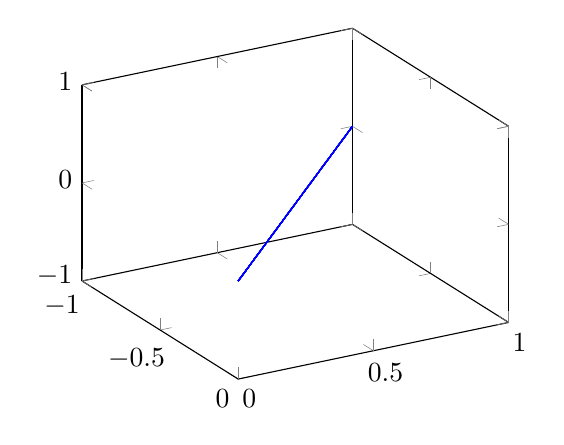
\begin{tikzpicture}
    \begin{axis}[view={60}{30}]
        \addplot3 [
            mesh,
            z buffer=sort,
            samples=20,
            domain=-1:0,
            y domain=0:2*pi,
        ] (
    {x},
    {-x},
    0
    );
    \end{axis}
    \end{tikzpicture} 
\end{center}
2) $U \cup U' \subseteq V$ n'est en général pas un sous-espace vectoriel de $V$.
Généralement, le plus petit sous-espace vectoriel contenant $U \cup U'$ est le sous-espace vectoriel noté $U + U'$ appelé \textbf{somme} de $U$ et $U'$, défini par :
$$
U +U ' = \{u+u' \quad | \quad u \in U, u' \in U'\}$$
On peut démontrer facilement que $U+U'$ est bien un sous-espace vectoriel de $V$.

\subsection{Propriétés des espaces vectoriels}
Soit $V$ espace vectoriel réel sur un corps $K$. Alors :
\begin{enumerate}
    \item L'élément neutre pour l'addition est unique.
    \item $\forall v \in V$, l'opposé est unique.
    \item $\mathbb 0_K \cdot v = \mathbb 0_V \quad \forall v \in V$ 
    \item $\alpha \cdot \mathbb 0_V = \mathbb 0_V \quad \forall \alpha \in K$
    \item Si $\alpha * v = \mathbb 0_V$ pour $\alpha \in K, v \in V$, alors $\alpha = \mathbb 0_K$ ou $v \in \mathbb 0_V$
    \item $\forall v \in V$, son opposé $-v$ satisfait $-v = (-1) * v \in K$
\end{enumerate}

\subsection{Preuves des propriétés}
\textbf{Propriété 1}
Soient deux éléments neutres $\zero_V, \zero_V'$ pour l'addition dans $V$.  On doit montrer que $\zero_V = \zero_V'$.
On a d'une part $\zero_V + \zero_V' = \zero_V$ car $\zero_V'$ est neutre. On a également $\zero_V + \zero_V' = \zero_V'$ car $\zero_V$ est neutre. On a donc $\zero_V = \zero_V'$.
\\
\textbf{Propriété 2}
Soient $-v, v'$ deux opposés de $v$. On doit montrer que $-v = v'$.
Puisque $v'$ est opposé de $v$, on a $v+v' = \zero$. Alors $(-v + v) + v' = -v + \zero = -v$. 
Donc $v'=-v$.
\\
\textbf{Propriété 3}
On doit montrer que $0_K * v = \zero_V$.
$0_K*v+v = 0_Kv+ 1_K *v = (0_K + 1_K)*v = 1_K*v = v \Rightarrow 0_K*v = \zero_V$.
\\
\textbf{Propriété 4}
Soit $v \in V$. Calculer $\alpha \cdot \zero_V + \alpha \cdot v = \alpha ( \zero_V + v) = \alpha \cdot v$
Donc puisque $\zero_V$ est l'élément neutre pour l'addition, $\alpha \cdot \zero_V = \zero_V$.
\\
\textbf{Propriété 5}
Supposons $\alpha *v = \zero_V$. Si $\alpha \neq 0_K$, alors on peut diviser par $\alpha$:
$\frac 1 \alpha * \alpha * v = \frac 1 \alpha * \zero_V = \zero_V \Rightarrow v = \zero_V$
\\
\textbf{Propriété 6}
Montrons que $-v = (-1)_K*v$.
Puisqu'on a montré que $-v$ est l'unique opposé de $v$, il suffit de montrer que $-1*v$ est un opposé de $v$.
$-1*v + v = -1 * v + 1 * v = v * (1 - 1) = v*0_K = \zero_V$. Puisque l'inverse est unique, on a bien $-1*v = -v$.

\section{Chapitre 2 - Groupes, anneaux et corps}
\subsection{Définition - Groupe}
Un \textbf{groupe} est un ensemble $G$ muni d'une opération binaire :
$$
G \times G \rightarrow G, \quad a,b \rightarrow a \cdot b
$$
satisfaisant les axiomes d'associativité, possédant un élément neutre, que tout élément aie un inverse. 
Si l'opération est en plus commutative $(g \cdot h = h \cdot g)$ alors on dit que le group est \textbf{abélien}.
\pagebreak
\subsection{Définition - Anneau}
Un \textbf{anneau} est un ensemble $A$ muni de deux opérations binaires :
$$
+ : A \times A \rightarrow A, \quad a,b \rightarrow a + b
$$
$$\cdot : A \times A \rightarrow A, \quad a,b \rightarrow a\cdot b$$
$(A, +)$ est un groupe abélien. 
La multiplication est associative et il existe un élément neutre pour la multiplication ($1$). 
La distributivité est vérifiée ($(a+b)\cdot c = ac + bc$).
Si la multiplication est commutative, on parle d'anneau commutatif. $\mathbb Z$ est un anneau commutatif. $\mathbb M_2(\R)$ est un anneau non-commutatif, puisque la multiplication de matrices n'est pas commutative.

\subsection{Définition - Corps}
Un \textbf{corps} est un anneau commutatif $K$ tel que $0 \neq 1$. (l'élément neutre pour l'addition n'est pas le même que l'élément neutre pour la multiplication) non-nul de $K$ possède un inverse pour la multiplication.
On peut aussi dire qu'un corps est un ensemble $K$ muni de deux opérations $+$ et $\cdot$, tel que
\begin{itemize}
    \item ($K, +$ ) est un groupe abélien avec l'élément neutre noté $0$
    \item $(K \backslash \{0\}, \cdot)$ est un groupe abélien avec l'élément neutre  noté $1$ et tel que la distributivité est vérifiée.
\end{itemize}
Le corps $\C$ des nombres complexes nous intéresse en particulier.

\subsection{Définition - Complexes}
On définit $\C$ tel que :
$$ \C = \{a+ib \quad a,b \in \R \text{ et } i^2 = -1\}$$
On note $z=a+ib$.
$a$ est la partie réelle de $z$ et $b$ sa partie imaginaire. On représente souvent les nombres complexes sur le plan, avec leur partie réelle en abscisse et leur partie imaginaire en ordonnée. On peut donc définir un argument et un module.



\subsubsection{Module de z}
On écrit le module d'un nombre complexe $z$ comme suit :
$$|z| = \sqrt{a^2+b^2}$$
Géométriquement, il correspond à la longueur du vecteur sur le plan des complexes.

\subsubsection{Argument de z}
$$arg(z) = \alpha \text{ l'angle entre l'axe x et le vecteur z}$$

\subsubsection{Coordonnées polaires}
On peut écrire $z$ en coordonnées polaires :
$$z = (r, \alpha)$$
avec $r=|z|$ et $\alpha = arg(z)$.

On peut aussi écrire :
$$z = r \cdot (\cos \alpha + i \sin \alpha)$$
La notation d'Euler est la suivante et est équivalente :
$$
z = r \cdot e^{i \alpha}
$$

\subsubsection{Parties réelles et imaginaires}
On note $z = Re(z) + Im(z)*i$ avec $Re(z) = r \cos \alpha$, $Im(z) = r \sin \alpha$.
Il est à noter que $Re(z), Im(z) \in \R$ et pas $\C$.

\subsubsection{Conjugué de z}
Le conjugué de $z = a + bi$ est égal à $\bar z = a - bi$.
Il a plusieurs propriétés :
\begin{itemize}
    \item $\bar{z+w} = \bar z + \bar w$
    \item $\bar{z \cdot w} = \bar z \cdot \bar w$
\end{itemize}

\subsubsection{Inverse de z}
On peut calculer l'inverse de $z$ comme suit :
$$
z^{-1} = \frac{\bar z}{|z|^2}
$$
\subsubsection{Preuve de l'inverse de z}
On veut démontrer $z * \bar z = |z|^2$, donc que $z*\frac{\bar z}{|z|^2}=1$.
Puisque 1 est l'élément neutre de la multiplication dans $C$, $\frac{\bar z}{|z|^2}$ est bien l'inverse de $z$.

\subsection{Théorème - C est un corps}
$\C$ muni des opérations d'addition et de multiplication de nombres complexes est un corps.
\subsubsection{Preuve - C est un corps}
$(\C, +)$ possède le neutre $0$. C'est un groupe abélien.
$(\C \backslash \{0\}, \cdot)$ est un groupe par le Corollaire. On peut vérifier
que ce groupe est aussi abélien. Et la distributivité est aussi vérifiée.

\[
\begin{aligned}
    (a+bi) + (c + di ) &= (a+c) + (b+d)i
     \\
     (a+bi) \cdot (c + di) &= (ac-bd) + (ad+bc)i
\end{aligned}
\]
Ainsi, on peut établir :
\[
\begin{aligned}
    Re(z + z') = Re(z) + Re(z')
     \\
    Im(z + z') = Im(z) + Im(z')
\end{aligned}
\]
\end{document}